\begin{tcolorbox}
\chapter{2007 - The Final Nameless Expo}
An absolutely stonking year! We were very lucky with the weather, together with lots of interesting developments. No accidents, no missed call outs and generally a very smoothly run, pleasant and safe expedition.

The \passage{Captain Kangaroo} branch of \passage{Gardeners' World} was pushed to within 28 m of the lower \passage{M2} 1980s JSPDT survey. There is a possibility that we are unknowingly connected, as the Slovenes did not use PSSs in the 1970s except for a red paint splodge at the bottom of \passage{Silos}, and there's a probability that a connection exists.

Combined, the two cave systems would be 16722 m long (11493 m + 5229 m) - the second longest system in Slovenia\ldots{}

The connection will be a major target for 2008, with the possibility mooted of rigging down \passage{M2}.



\end{tcolorbox}
\backgroundsetup{
    scale=1.1,
    color=black,
    opacity=1,
    angle=0,
    contents={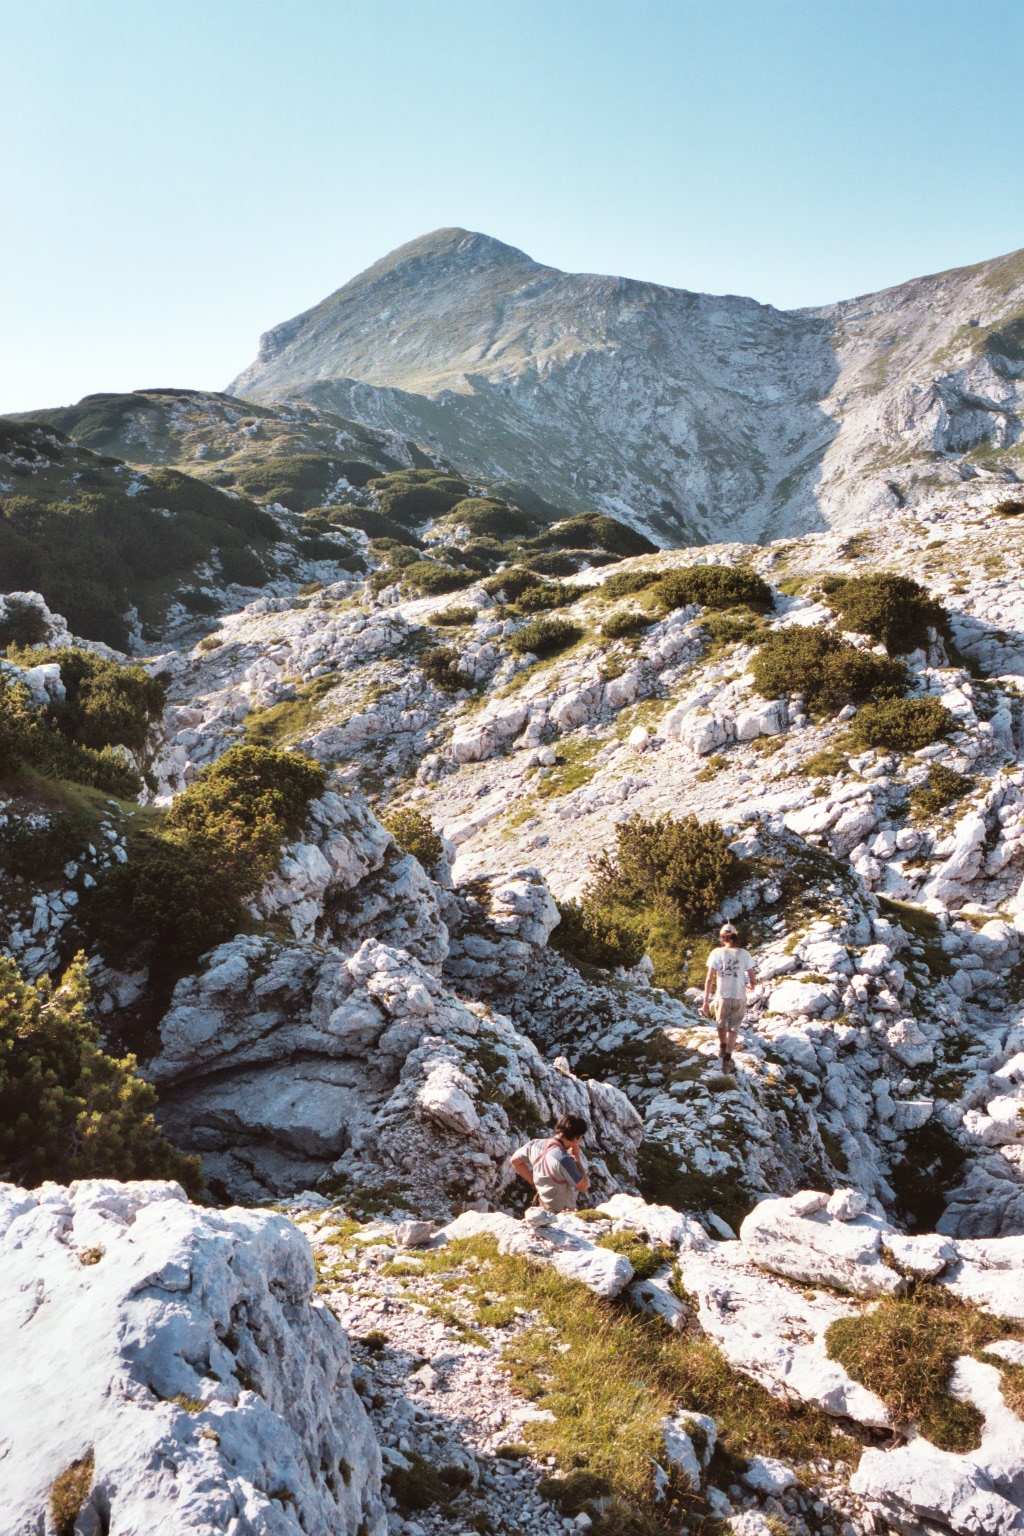
\includegraphics[height=\paperheight]{2007/intro/jarvist frost gr1 film1 -027_24--orig.jpg}}
}
\BgThispage
